% !TEX options=--shell-escape
\documentclass[usenames,dvipsnames,9pt]{beamer}

\makeatletter
\def\input@path{{support/beamer-template/}}
\makeatother

\usepackage{support/beamer-template/beamerthememetropolis}

\usepackage[utf8]{inputenc}
\usepackage[czech]{babel}
\selectlanguage{czech}

\usepackage{hyperref}
\usepackage{fontawesome}
\usepackage{minted}
\usepackage{mathtools}
\usepackage{tabularx}
\usepackage{smartdiagram}
\usepackage{amssymb}
\usepackage{qrcode}

% Commands shared between most of the tutorial slides

% Homework deadlines
\newcommand{\hwVIIdeadline}{10. 5. 2020}



% Download icon and text with link relative to the root of the courseware site
\newcommand{\download}[1]{\hfill\faDownload\hspace{5pt}\href{https://cw.fel.cvut.cz/wiki/_media/courses/be4m36mas/#1}{\tt #1}\\[1.3em]}

% Draw eye icon
\newcommand{\see}[1]{\faEye\hspace{5pt}#1}

\newcommand{\sep}{\hspace{10pt}/\hspace{10pt}}

\def\Ipe#1{\def\IPEfile{#1}\input{#1}}

% Draw pacman icon
\newcommand{\pacman}[1]{\tikz[baseline=.1em,scale=.6]{
    \useasboundingbox (.02,0) rectangle (.6,.6);
  \draw [fill=#1] (.3,.3) -- ++(25:.3) arc (+25:+335:.3) -- cycle;

}}

% Draw ghost icon
\newcommand{\ghost}[1]{\tikz[baseline=.1em,scale=.5]{
  \draw [fill=#1] (0,0) -- (0,.5) arc (+180:0:.3) -- (.6,0) --
  (.5,.15) -- (.4,0) -- (.3,.15) -- (.2,0) -- (.1,.15) -- cycle;
    \coordinate (eye) at (360*rand:.03);
    \foreach \x in {.17,.43}{
      \fill[white] (\x,.5) circle[radius=.1];
      \fill[black] (\x,.5) ++(eye) circle[radius=.05];
    }
}}

\newcommand{\desc}[2]{
  #1

  \vspace{-0.6em}
  \hfill\begin{minipage}{0.9\linewidth}
    #2
  \end{minipage}

  \vspace{0.2em}
}

\newcommand{\redc}{\tikz\draw[red,fill=red] (0,0) circle (.5ex);}

\newcommand{\greenc}{\tikz\draw[green,fill=green] (0,0) circle (.5ex);}


% Default url for generating QR code with feedback form.
\newcommand{\defaultfeedbackurl}{https://forms.gle/vwbWazEu14w1Kf487}

% Generate frame with QR code to a feedback form.
\newcommand{\framefeedback}[1][\defaultfeedbackurl]{
  \begin{frame}[standout]
    \begin{minipage}{0.4\linewidth}
      \begin{center}
        \textbf{\LARGE Díky za pozornost!}
      \end{center}

      \vspace{3em}

      \raggedleft\small Budeme rádi za Vaši\\zpětnou vazbu! $\rightarrow$
    \end{minipage}
    \hfill
    \begin{minipage}{0.5\linewidth}
      \vspace{4em}
      \centering\qrcode[height=\linewidth]{#1}\\
      \vspace{0.8em}
      \url{#1}
    \end{minipage}
  \end{frame}
}

\title{Řadící algoritmy}
\date{}
\institute{B4B36PDV -- Paralelní a distribuované výpočty}

\metroset{block=fill}

\begin{document}
\maketitle

\begin{frame}
  \frametitle{Osnova}
  \begin{itemize}
    \item Opakování z minulého cvičení\\[1.5em]
    \item Dynamické vytváření úloh s \#pragma omp task
    \item Paralelní merge sort
    \item Paralelní counting sort\\[1.5em]
    \item Zadání páté domácí úlohy
  \end{itemize}
\end{frame}


\section{Opakování z minulého cvičení}

\begin{frame}[standout]
  \Huge
  \url{http://goo.gl/a6BEMb}
\end{frame}

{\setbeamertemplate{frame footer}{\see{\url{http://goo.gl/a6BEMb}}}
\begin{frame}[fragile]
\frametitle{Co můžete říct o tomto kódu?}

  \begin{minted}{c}
#pragma omp parallel
#pragma omp for
for(int i = 0 ; i < size ; i++) {
  if(is_solution(candidates[i])) {
    std::cout << candidates[i]
              << "is a solution" << std::endl;
    break;
  }
}
  \end{minted}
  
  \vspace{.3em}
  
  \begin{itemize}
  \item Nepůjde pravděpodobně zkompilovat
  \item Paralelní blok skončí po nalezení prvního řešení
  \item Paralelní blok skončí, až všechna vlákna najdou řešení
  \item Aby blok skončil ihned po nalezení řešení, musíme (vhodně) doplnit \texttt{\#pragma omp cancel for}
  \item Aby blok skončil ihned po nalezení řešení, musíme (vhodně) doplnit \texttt{\#pragma omp cancelation point for}
  \item Měli bychom nastavit proměnnou prostředí \texttt{OMP\_CANCELLATION=true}
  \end{itemize}

\end{frame}

\begin{frame}[fragile]
\frametitle{Jak se bude chovat následující kód?}

  \begin{minted}{c}
int parallel_worker(int d){
  if (d == 1) return 1;
  int t1 = 0, t2 = 0;
  #pragma omp task
  t1 = parallel_worker(d-1);
  #pragma omp task
  t2 = parallel_worker(d-1);
  #pragma omp taskwait
  return t1+t2;
}
(...)
#pragma omp parallel num_threads(4)
std::cout << parallel_worker(3) ;
  \end{minted}

\end{frame}
}


\section{\texttt{\#pragma omp task}}

\begin{frame}[fragile]
	\frametitle{\texttt{\#pragma omp task}}
	Pokud nevíme, jaké úlohy budeme muset v průběhu výpočtu řešit, můžeme je vytvářet dynamicky...

	\begin{minted}{c}
void traverse(node * n) {
  for(node * successor : n->getSuccessors()) {
    #pragma omp task
    traverse(successor);
  }

  do_something();
  
  #pragma omp taskwait
}
 	\end{minted}
\end{frame}

\begin{frame}[fragile]
	\frametitle{\texttt{\#pragma omp task}}
	Co kdybychom chtěli z tasků ale něco vracet?

	\begin{minted}{c}
unsigned long long traverse_and_sum(node * n) {
  std::atomic<unsigned long long> sum = 0;
  for(node * successor : n->getSuccessors()) {
    #pragma omp task shared(sum)
    sum += traverse(successor);
  }

  sum += do_something(n);
  
  #pragma omp taskwait
  return sum.load();
}
 	\end{minted}

	\faWarning \hspace{2pt} \textbf{Pozor!} Nutno použít \texttt{shared} (pro přístup k proměnné) a \texttt{taskwait}!
	Nepoužití těchto konstruktů povede k špatnému výsledku programu (data se nezapíší globálně) nebo i k pádu (proměnná \texttt{sum} zanikne po \texttt{return})!
\end{frame}

\begin{frame}[fragile]
	\frametitle{\texttt{\#pragma omp task}}
	Něco nám tam ale chybí... Ještě potřebujeme ,,někoho``, kdo \texttt{tasky} bude řešit. Potřebujeme si připravit vlákna!

	\begin{minted}{c}
unsigned long long start_traversal() {
  #pragma omp parallel   // Vytvoříme si tým vláken
  traverse_and_sum(root);
}
 	\end{minted}

 	\pause
 	\vspace{2em}\hrule\vspace{1em}

 	\large\textbf{Rychlá otázka:} Stane se skutečně to, co bychom chtěli?
\end{frame}

\begin{frame}[fragile]
	\frametitle{\texttt{\#pragma omp task}}
	My ale chceme, aby kořen zpracovávalo pouze \underline{jedno} vlákno!

	\vspace{2em}

	\begin{minted}{c}
unsigned long long start_traversal() {
  #pragma omp parallel
  #pragma omp single     // pouze jednou!
  traverse_and_sum(root);
}
 	\end{minted}

 	\pause
 	\vspace{1em}\hrule\vspace{1em}

 	\large\textbf{Rychlá otázka:} Stane se skutečně to, co bychom chtěli?
\end{frame}

\begin{frame}[fragile]
	\begin{center}
		\Large\faWarning \hspace{2pt} Režie s vytvářením a správou \texttt{tasků} může být drahá. \\
	\end{center}
	\begin{itemize}
		\item Tasky chceme vytvářet tehdy, pokud to povede k lepšímu vytížení procesoru.
		\item ... ale ne nutně výhradně spravováním tasků ;-)
	\end{itemize}

	\vspace{1em}\hrule\vspace{1em}

	\begin{minted}{c}
double x = 0.0;
if(size <= MIN_PROBLEM_SIZE) {
	return solve_sequential(...);
} else {
	#pragma omp task shared(x)
	x += task1(x);

	#pragma omp task shared(x)
	x += task2(x);

	#pragma omp taskwait
	return x;
}
 	\end{minted}
\end{frame}

\begin{frame}[fragile]
\frametitle{Příklad \texttt{\#pragma omp task}: Paralelní suma}

\begin{minted}{c}
float sum(const float *a, size_t n){
    float r;
    #pragma omp parallel
    #pragma omp single
    r = parallel_sum(a, n);
    return r;
}

static float parallel_sum(const float *a, size_t n){
    if (n <= CUTOFF) { return serial_sum(a, n);}
    float x, y;	size_t half = n / 2;
    #pragma omp task shared(x)
    x = parallel_sum(a, half);
    #pragma omp task shared(y)
    y = parallel_sum(a + half, n - half);
    #pragma omp taskwait
    x += y;
    return x;
}
  \end{minted}
  
\end{frame}

\section{Paralelní merge sort}

\begin{frame}[fragile]
\frametitle{Paralelní merge sort}

Merge sort je řadící algoritmus, který pracuje následovně:

\begin{enumerate}
\item Rozdělí neseřazenou množinu dat na dvě podmnožiny o přibližně stejné velikosti.
\item Seřadí obě podmnožiny.
\item Spojí seřazené podmnožiny do jedné seřazené množiny.
\end{enumerate}

\vspace{1em}\hrule\vspace{1em}

\begin{minted}{c}
function mergesort(m)
    if (length(m) <= 1) return m

    middle = length(m) / 2
    left = m[0 ... middle-1]
    right = m[middle ... length(m)-1]

    left = mergesort(left)
    right = mergesort(right)

    return merge(left, right)
\end{minted}

  
\end{frame}

\begin{frame}[fragile]
\frametitle{Paralelní merge sort}

\begin{center}
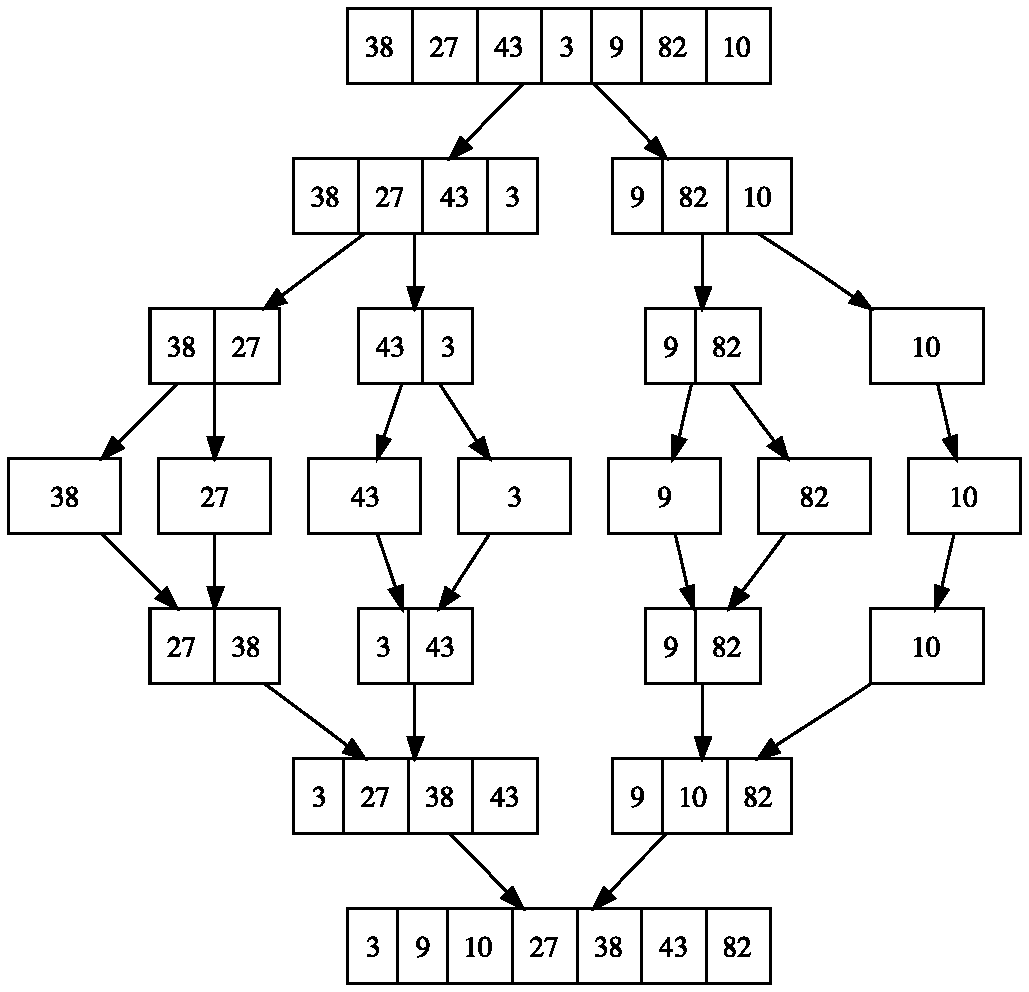
\includegraphics[width=.7\linewidth]{06/figs/mergesort.pdf}
\end{center}

  
\end{frame}


{\setbeamertemplate{frame footer}{\see{{\tt mergesort\_parallel.h}, {\tt sorting.cpp} }}
\begin{frame}[fragile]
\frametitle{Paralelní merge sort}

  \begin{block}{Doimplementujte metodu \texttt{mergesort\_parallel}}
    Doimplementujte tělo metody \texttt{mergesort\_parallel(...)} (a případných dalších metod, které budete potřebovat) v souboru \texttt{mergesort\_parallel.h}.
    Pro implementaci můžete využít metodu \texttt{merge(...)} a můžete se inspirovat sekvenční implementací, kterou naleznete v souboru \texttt{mergesort\_sequential.h}.
  \end{block}
  
  \vspace{2em}
  
  \begin{center}
  	\large \faWarning \hspace{3pt} Proměnné v \texttt{task} jsou privátní (\texttt{lastprivate}) pro daný task, pokud neřeknete jinak (pomocí parametru OpenMP \texttt{shared(x)}).
  \end{center}
  
\end{frame}

\begin{frame}
	\textbf{Otázka:} Jakou složitost má sekvenční mergesort? A jak je na tom jeho paralelní verze?
\end{frame}
}

\section{Paralelní counting sort}

{\setbeamertemplate{frame footer}{\see{{\tt countingsort.h}, {\tt sorting.cpp} }}
\begin{frame}
	\frametitle{Counting sort}
	Uvažujme, že máme za úkol seřadit pole prvků, které obsahuje hodnoty z malého omezeného rozsahu $a \leq x \leq b$.

	Pak může být použití standartních algoritmů se složitostí $O(n \log n)$ nevhodné.

	\vspace{1em}\hrule\vspace{1em}

	\textbf{Counting sort:}
	\begin{enumerate}
		\item Napočítáme si počty jednotlivých prvků $c(x)$ z rozsahu $x\in[a,b]$ (,,histogram``)
		\item Počty prvků projdeme ve vzestupném pořadí. Prvek $x$ zapíšeme do výstupního pole $c(x)$-krát.
	\end{enumerate}

	\vspace{1em}

	\hfill $\rightarrow$ Složitost $O(n + k)$, kde $k = b-a+1$
\end{frame}
\begin{frame}
	\frametitle{Counting sort}
	\begin{enumerate}
		\item Napočítáme si počty jednotlivých prvků $c(x)$ z rozsahu $x\in[a,b]$ (,,histogram``)
		\item Počty prvků projdeme ve vzestupném pořadí. Prvek $x$ zapíšeme do výstupního pole $c(x)$-krát.
	\end{enumerate}

	\vspace{1em}\hrule\vspace{1em}

	\begin{center}
		\Large Jak bychom kroky 1 a 2 mohli paralelizovat?
	\end{center}

	\pause

	\begin{block}{Doimplementujte metodu \texttt{counting\_parallel}}
	    Doimplementujte tělo metody \texttt{counting\_parallel(...)} v souboru \texttt{countingsort.h}.
	    Inspirovat se můžete sekvenční implementací tohoto řadícího algoritmu v metodě \texttt{counting\_sequential(...)}
    \end{block}
\end{frame}

\begin{frame}[standout]
	\LARGE \faWarning \hspace{2pt} SPOILER ALERT!
\end{frame}

\section{Prefixní suma}

\begin{frame}[fragile]
	\begin{enumerate}
		\item Napočítáme si počty jednotlivých prvků $c(x)$ z rozsahu $x\in[a,b]$ (,,histogram``)
		\item Počty prvků projdeme ve vzestupném pořadí. Prvek $x$ zapíšeme do výstupního pole $c(x)$-krát.
	\end{enumerate}

	\vspace{1em}\hrule\vspace{1em}

	\begin{center}
		\large Bod (2) algoritmu nešel snadno paralelizovat, protože nevíme, kam máme dané číslo umístit bez toho, abychom vyřešili předešlá čísla!
		\[ c(x) = [ \textcolor{red}{?}, \ \, \textcolor{red}{?},\ \ 5,\ \ \textcolor{red}{?}, \ \, \textcolor{red}{?}] \]
	\end{center}

	\hfill $\rightarrow$ Pojďme to vyřešit...
\end{frame}

\begin{frame}
\frametitle{Prefixní suma}

Pro posloupnost čísel $x_0, x_1, x_2, \dots$ je prefixní suma posloupnost $y_0, y_1, y_2, \dots$ taková, že

\begin{align*}
y_0 &= x_0 \\
y_1 & = y_0 + x_1\\
y_2 & = y_1 + x_2\\
&~\vdots
\end{align*}

\vspace{1em}\hrule\vspace{1em}

{\bf Příklad:}

\begin{tabular}{ l c c c c c c c }
  Vstupní sekvence: 	& 1 & 2 & 3 & 4 & 5 & 6 & \dots \\
  Prefixní suma:		& 1 & 3 & 6 & 10 & 15 & 21 & \dots  \\
\end{tabular}

\end{frame}

{\setbeamertemplate{frame footer}{\see{{\tt countingsort.h}, {\tt sorting.cpp} }}
\begin{frame}
	\begin{block}{Doimplementujte metodu \texttt{counting\_parallel}}
	    Použijte prefixní sumu pro paralelizaci bodu (2) counting sortu.
    \end{block}
\end{frame}}

{\setbeamertemplate{frame footer}{\see{{\tt prefixsum.h}, {\tt prefixsum.cpp} }}
\begin{frame}
\frametitle{Prefixní suma}

	\begin{center}
		\Large Jak bychom mohli výpočet prefixní sumy paralelizovat? \\
		\large Hodnota $y_i$ stále závisí na hodnotě $y_{i-1}$
	\end{center}

  \begin{block}{Doimplementujte metodu \texttt{prefix\_sum\_parallel}}
    Doimplementujte tělo metody \texttt{prefix\_sum\_parallel} v souboru \texttt{prefixsum.h}.
  \end{block}
\end{frame}
}
}


 \section{Zadání páté domácí úlohy}
 
% \begin{frame}
%   \frametitle{Paralelní radix sort}
%
%
%
% \end{frame}
 
 

 \begin{frame}
   \frametitle{Paralelní radix sort}
   
   Algoritmus pro lexikografické seřazení řetězců stejné délky.
   
      \vspace{1.5em}
   
   Naimplementujte metodu \texttt{radix\_par} v \texttt{sort.cpp}.% a zajistěte, že
 %  \begin{enumerate}
 %    \item každý prvek je vložet právě jednou; a
 %    \item žádný vložený prvek se neztratí.
 %  \end{enumerate}
  
  
   \vspace{1.5em}
  
   Za správné výsledky a rychlé zpracování dostanete až {\bf 2b}.
  
    \vspace{1.5em}
    
   

 Soubory \texttt{sort.cpp} a \texttt{sort.h}  nahrajte do systému BRUTE.
  

 \end{frame}


% Frame with the feedback QR code 
\framefeedback{}

\end{document}
